\documentclass[draft]{agujournal2019}
\usepackage{url} %this package should fix any errors with URLs in refs.
\usepackage{lineno}
\usepackage[inline]{trackchanges} %for better track changes. finalnew option will compile document with changes incorporated.
\usepackage{soul}
\usepackage{lscape}
\usepackage{rotating}
\usepackage{longtable}
\linenumbers

\draftfalse

\journalname{Geochemistry, Geophysics, Geosystems}

%%%%Version 3 edits on 9/24 ish: removed the written communication reference and added the Geologic materials center as the source for the samples. Specified in selected places in the text that descrpitions and sample material were from the GMC.

%%%% Version 4 edits on 10/6/21: added the MAGIC URL to the text and acknowledgements section, and added  a statement to the acknowledgements for the github repository archive and url


\begin{document}


\title{New paleointensity data from Aniakchak volcano, Alaska, USA}


\authors{Geoffrey Cromwell\affil{1}\affil{2} and Yiming Zhang\affil{1}\affil{3}}

\affiliation{1}{Occidental College, Los Angeles, CA, USA}
\affiliation{2}{Current Address: U.S. Geological Survey, California Water Science Center, Santa Maria, CA, USA}
\affiliation{3}{Current Address: University of California Berkeley, Berkeley, CA, USA}

\correspondingauthor{Cromwell, G.}{geoffrey.cromwell@gmail.com, gcromwell@usgs.gov}

\begin{keypoints}
\item We report the first set of absolute paleointensity data from Aniakchak volcano, Alaska, USA.
\item Glassy volcanic material yield high-quality results and were evaluated using strict-selection criteria
\item The new data fill in a gap of Holocene-age absolute paleointensity records from mid- to high-latitudes in North America
%\item This study reports new robust paleointensity data from a new location of Aniakchak volcano, Alaska that suggest a persistent field structure near northern Pacific region over the past three thousand years which has not been predicted by previous models. 
%\item Rapidly cooled volcanic glass materials coupled with strict paleointensity methods can enrich the current paleointensity databases with great potentials of overcoming the disadvantages of archaeomagnetic and sedimentary sources. 
\end{keypoints}


\begin{abstract}
This study presents the first set of Holocene-age, high-quality absolute paleointensity data from Alaska, USA. Existing paleointensity data for the Holocene are generally located at mid-northern latitudes in North America, Europe, the Middle East, and eastern Asia. Relatively few data are from the Alaska region. IZZI-modified paleointensity experiments were conducted on glassy volcanic materials from Aniakchak volcano, a mid- to high-latitude composite volcano on the Alaska-Aleutian arc. %The IZZI-Thellier paleointensity technique was used to derive absolute paleointensity estimates using glassy volcanic materials collected from U.S. Geological Survey archives in Anchorage, Alaska. 
The CCRIT selection criteria were applied to the paleointensity results. A total of 30 specimens from six samples with estimated ages ranging from 1931 C.E. to 2,300 years before present passed all selection criteria. The sample-mean paleointensities ranged from about 49 to 68 microTesla ($\mu$T). The sample-mean paleointensity results are comparable to modeled intensities, however all except for one sample-mean paleointensity are lower than those predicted by geomagnetic field models. The paleointensity estimate for the historic 1931 C.E. eruption was about 15 $\mu$T greater than the expected field strength. This overestimate may result from unrecognized alteration or non-ideal remanence carriers in this sample. Further evaluation of samples from the 1931 C.E. eruption using a Bayesian estimation method resulted in a paleointensity estimate that encompasses the historical field strength within uncertainty. These new paleointensity results are a valuable contribution to the mid- to high-northern latitude paleomagnetic dataset. Incorporation of these data into future geomagnetic field models will improve the predictions of geomagnetic field behavior in the Alaska region.
\end{abstract}


\section{Introduction}
Reconstructing the Holocene evolution of Earth's magnetic field is important for understanding geodynamo processes in Earth's core, for studying long-term solar-terrestrial relationships, and for providing useful age constraints for archeological and stratigraphic units. Currently there are several observation-based, continuous global geomagnetic field models \cite{Constable2016a,Korte2009a,Korte2011a,Korte2011b,Pavon-Carrasco2014a,Nilsson2014a} that have various reconstructions and predictions of paleodirection and absolute paleointensity using historic measurements of the geomagnetic field and paleomagnetic data from archeomagnetic, volcanic, and sedimentary materials. Depending on the availability of spatially and temporally distributed reliable paleomagnetic data, the accuracy and resolution of different models of the past geomagnetic field can vary. Currently the majority of the Holocene archeomagnetic and volcanic paleointensity data come from mid-northern latitudes ($30^{\circ}$N to about $50^{\circ}$N) in North America, Europe, the Middle East, and eastern Asia \cite{Brown2015a, Brown2015b}, biasing the models toward better resolution in these regions and lower resolutions in the higher latitudes and in the southern hemisphere. To improve future geomagnetic field models, it is essential to add more high-quality paleomagnetic data from areas with few current data points.

An under-represented region in the current paleomagnetic  database is Alaska, especially along the volcanically active Alaska-Aleutian arc. Previous paleomagnetic studies in Alaska  have mostly focused on tectonic questions on mainland Alaska \cite{Packer1974a,Hillhouse1980a,Thrupp1986a,Stamatakos2001a}, or paleosecular variation studies on volcanoes along the Alaska-Aleutian arc \cite{Stone1979a,Bingham1972a,Stone2006a} and on Nunivak Island \cite{Coe2000,Johnson2008a}. Paleointensity records from Alaska are limited, especially absolute paleointensity records. Previous studies focused on determining the relative paleointensity records from sediment cores with the purpose of better constraining the regional chronostratigraphy of the western Arctic \cite{Barletta2008a, Lise-Pronovost2009a}. \citeA{Stone2006a} conducted absolute paleointensity experiments using Thellier-Coe method \cite{Coe1967b} on lava flows from the Aleutian Islands. However, only two samples from a \textit{ca.} 2 Ma lava flow and one sample from a \textit{ca.} 50 ka lava flow yielded acceptable paleointensity results. An evaluation of the efficacy of paleointensity experiments on pyroclastic-flow material from the historical 1912 C.E. Novarupta volcano was conducted by \citeA{Bowles2015b}.  Sparse temporal coverage, and low success rate for absolute paleointensity records have limited  systematic interpretation of the geomagnetic field behavior over the Alaska-Aleutian arc region.

Nevertheless, volcanoes of the Alaska-Aleutian arc are promising targets for northern mid- to high-latitude paleointensity investigations because of the active volcanism along the arc, availability of detailed geologic maps, and the preservation of fresh, glassy volcanic materials which can be faithful paleointensity recorders \cite{Cromwell2015a, Cromwell2015b, Cromwell2018a}. Aniakchack volcano, an active Pleistocene-Holocene composite volcano, is one such target (Figure \ref{Geologic_map}). The volcano has undergone at least one caldera-forming eruption in postglacial time and last erupted in 1931 C.E. \cite{Bacon2014a}. Aniakchak volcano contains glassy volcanic materials and has an established stratigraphic record that is calibrated based on $^{14}$C radiocarbon geochronology constraints from organic materials within or between eruptive materials \cite{Bacon2014a}. To date, no paleomagnetic studies have been conducted on Aniakchak volcano. 

Glassy volcanic materials from Aniakchak can be ideal targets for paleointensity experiments because single domain stable magnetic minerals tend to form during rapid cooling and often yield ideal paleointensity behaviors \cite{Tauxe2004a,Dunlop2005a}. A previous paleointensity study successfully obtained high-quality paleointensity estimates using submarine basaltic glass as old as 92 Ma \cite{Tauxe2004a}. More recent paleointensity studies on young (centuries to tens of thousands of years), fresh, glassy volcanic materials, formed from sub-aerial and sub-glacial eruptions, have accurately recovered geomagnetic field strengths that match with modeling results \cite{Cromwell2015a, Cromwell2015b, Cai2017a, Cromwell2018a}. In this study, we conduct IZZI-modified paleointensity experiments \cite{Tauxe2004b} on glassy volcanic materials from Aniakchak volcano. Our data add to the observational records of the geomagnetic field strength at mid- to high-northern latitudes in Alaska during the Holocene.

\begin{figure}
\centering
\noindent\includegraphics[width=40pc]{../Figure/Aniakchak_geologic_map_092421.pdf}
\caption{Regional setting of Aniakchak volcano. A) Location of Aniakchak volcano with respect to the State of Alaska, USA, the city of Anchorage, and municipal boundaries; B) perspective view of Aniakchak volcano (GoogleEarth imagery); C) Geologic map of Aniakchak caldera with locations of paleointensity sample used in this study, modified from \protect\citeA{Bacon2014a}.}
\label{Geologic_map}
\end{figure}

\section{Geologic Setting}

The Alaska-Aleutian arc is an active chain of volcanoes that formed in the Eocene \cite{Jicha2006a} as a result of subduction of the Pacific Plate under the North American Plate. Aniakchak volcano (located at approximately 56.9 $^{\circ}$N, -158.2 $^{\circ}$E) is a Pleistocene-Holocene composite volcano located in the eastern part of the Alaska–Aleutian arc on the Alaska Peninsula, about 670 km southwest of Anchorage, Alaska (Figure \ref{Geologic_map}). Aniakchak has been an active volcano since the last glacial period, having experienced multiple sub-Plinian to Plinian eruptions. The earliest Holocene Aniakchak eruption has been dated with radiocarbon method to have occurred between \textit{ca.} 9,500 and 7,000 years ago before present (yrs B.P.; \citeA{Vanderhoek2009a}), and the latest eruption was a sub-Plinian eruption in 1931 C.E. 

Aniakchack volcano has been the subject of several geologic investigations, the most comprehensive one being a report on the postglacial eruption history, geochemistry and recent seismicity of the volcano by \citeA{Bacon2014a}. \citeA{Bacon2014a} built upon previous investigations of the eruptive history of the volcano \cite{Miller1977a,Miller1987a,Neal1992a,Vanderhoek2004a,Vanderhoek2009a}, specific eruptive and geologic events \cite{Beget1992a,McGimsey1994a}, potential volcanic hazards \cite{Neal2001a}, and the geochemistry, petrology and magma evolution of the volcano \cite{George2004a,Dreher2005a,Symonds2003a}. A study by \citeA{Pearce2017a} uses tephra from a radiocarbon-dated Aniakchak eruption to constrain the chronology of submarine sediments. The earliest reports specific to Aniakchak were by \citeA{Smith1925a}, who published the first geologic map of the crater, and by \citeA{Hubbard1931a}, who visited Aniakchak before and after the historical 1931 C.E. eruption. This investigation of paleointensity will be the first paleomagnetic investigation of Aniakchak volcano.

Aniakchak volcano has had two major postglacial eruptions \cite{Miller1987a}. Aniakchak I is the oldest known eruption and the age of its andesite ignimbrite deposits has been bracketed by the timing of deglaciation around 9,500 yrs B.P. and $^{14}$C ages of \textit{ca.} 7,000 yrs B.P. of organic materials beneath stratigraphically younger pumice-fall deposits \cite{Vanderhoek2009a}. The other major eruption, named Aniakchak II, is estimated to have occurred \textit{ca.} 3,430$\pm$70 yrs B.P. based on $^{14}$C ages of charcoal within an ignimbrite emplaced during the event \cite{Miller1987a, Bacon2014a}. The Aniakchak II event formed the outer boundary of the present-day Aniakchak caldera (Figure \ref{Geologic_map}). Multiple following eruptive events after the Aniakchack II eruption are summarized in detail by \citeA{Bacon2014a} and illustrated in Figure \ref{Geologic_map}. The post-Aniakchak II record is complicated by a caldera lake having been present for part of this period, and little information is known about the earliest postcaldera materials prior to the emplacement of the dacite domes (unit Qd; Figure \ref{Geologic_map}; \citeA{Bacon2014a}). From the oldest to youngest, \citeA{Bacon2014a} describe the post-Aniakchak II geologic history to consist of subaqueous lava effusions forming dacite domes and related lava (Qd), catastrophic draining of the caldera lake, subsequent hydromagmatic eruptions forming the tuff cones (Qtc), later effusive and explosive eruptions that resulted in the formation of lava and scoria from Vent Mountain (Qvm), Half Cone (Qhc, Qht, Qhl), and scoria from Blocky Cone (Qb). Finally, the 1931 C.E. eruption of tephra (Q3t) and lava flows (Q3l). Some of the post-Aniakchack II eruptive materials are overlain by glaciers and surficial deposits.

\section{Sample Collection}
Unoriented hand-samples were collected by the U.S. Geological Survey (USGS) Alaska Volcano Observatory in Anchorage, Alaska as part of an effort to document the eruption history of Aniakchack volcano, which included conducting $^{14}$C radiometric age dating of organic materials to provide chronological control for the stratigraphic sections of the volcano, and conducting detailed geochemical analyses to document the magmatic processes associated with Aniakchak eruptions \cite{Bacon2014a}. For this study, thirteen samples of those collected by the USGS were acquired for paleointensity experiments from the \citeA{GMC2015} in Anchorage, Alaska.  Sample location information, descriptions, geologic unit assignments, and age estimates are listed in Table \ref{tab:samples}. Age estimates for each sample were interpreted for this study, all other information in Table \ref{tab:samples} was previously  published in \citeA{Bacon2014a} or available from the \citeA{GMC2015}. The original sample names used by \citeA{Bacon2014a} and the \citeA {GMC2015} are retained in this study. The samples included in this study are post-Aniakchak II eruptive materials and range in age from \textit{ca.} 2,300 yrs B.P. to 1931 C.E.

\subsection{Stratigraphy and Age Constraints}
Age constraints for the samples included in this study were interpreted based on sample descriptions and stratigraphic and radiometric age constraints reported by \citeA{Bacon2014a}, or summarized therein. The estimated ages of volcanic deposits in Aniakchak volcano were acquired through $^{14}$C dating on organic materials found in between tephra layers and lava flows in addition to stratigraphic relationships \cite{Bacon2014a}. The interpreted age estimates for each sample are based on the geologic unit of each sample (Table \ref{tab:samples}); unit assignments for all samples are from \citeA{Bacon2014a}, except for samples NA02-10F and NA02-11F which are interpreted for this study based on their location information and descriptions. Additional evaluation of the geochemical data of \citeA{Bacon2014a} (Figure \ref{TAS_plot}) may help constrain the age of selected samples. Ages reported by \citeA{Bacon2014a}, and used in this study, are given in radiocarbon years before 1950 C.E. In this section we briefly describe the location, geologic unit, and estimated ages for each sample used in our paleointensity experiment. 

\subsubsection{Subaqueous Domes (unit Qd)}
Samples NA92-42D and NA02-10G were collected from the subaqueous domes and related lava flows (unit Qd; Figure \ref{Geologic_map}) which has an estimated age range of 2,300–1,860 yrs B.P. (Table \ref{tab:samples}). The subaqueous domes are the oldest known products of post-Aniakchak II caldera-forming volcanism that were effused in an ancient caldera lake, of which modern Surprise Lake is a remnant (Figure \ref{Geologic_map}; \citeA{Bacon2014a}). The ancestral caldera lake was estimated to have catastrophically drained prior to 1,860$\pm$30 yr B.P. based on radiocarbon ages on wood from above sediment near the Aniakchak River mouth of 1,860$\pm$30 yr B.P. \cite{Vanderhoek2004a,Bacon2014a}), thereby providing a minimum age constraint for emplacement of the subaqueous domes. A ca. 2,300 yr B.P. pumice fall (derived from a radiocarbon age of 2,300$\pm$80 yr B.P. from \citeA{Bacon2014a}) is tentatively considered by \citeA{Bacon2014a} to have preceded, or to be contemporaneous with the emplacement of the subaqueous domes, thereby providing a maximum age constraint for the subaqueous domes.

\subsubsection{Tuff Cone (unit Qtc)}
Sample NA94-5 was collected from Tuff Cone (unit Qtc; Figure \ref{Geologic_map}), which has an estimated age range of 900 to 1,860 yrs B.P. (Table \ref{tab:samples}; \citeA{Bacon2014a}). Radiocarbon dating of a soil above a tephra with Surprise Cone-like chemistry yielded a weighted mean age of 900$\pm$80 yr B.P. \cite{Bacon2014a}, which is interpreted to provide a minimum age constraint for the emplacement of the Tuff Cone unit. The tuff cones are thought to postdate catastrophic draining of the ancestral caldera lake (1,860$\pm$30 yr B.P.;\citeA{Vanderhoek2004a,Bacon2014a}) to their approximate elevation in the caldera. This age is interpreted as a maximum age constraint for the emplacement of the Tuff Cone unit. We therefore assign an age range of sample NA94-5 to be between 900 and 1,860 yrs B.P. 

The geochemical composition of sample NA94-5 may further constrain its emplacement age. Sample NA94-5 was collected east of Windy Cone and has a basaltic andesite geochemistry attribute (Figure \ref{TAS_plot}) that resembles the mafic eruption material of the Tuff Cone unit. The range of total alkaline silicate (TAS) compositions for all Tuff Cone samples collected by \citeA{Bacon2014a} (Figure \ref{TAS_plot}) indicates that there might have been a magmatic evolution of material from more felsic to more mafic compositions, perhaps similar to what was observed for the duration of the Aniakchak II caldera-forming eruption \cite{Bacon2014a}. If magmatic evolution occurred during the development of the Tuff Cones, the low-silica/high-mafic composition of NA94-5 could indicate that it was emplaced near the end of the Tuff Cone eruptive period and could be closer to the younger radiocarbon age constraint of 900$\pm$80 yr B.P. \cite{Bacon2014a}. However, without direct geochronologic constraints on the sample, we consider the age uncertainty of this sample to be 900–1,860 yr B.P. 

\subsubsection{Vent Mountain (unit Qvm)}
Samples NA97-25, NA94-2, NA97-24, and NA93-100A were collected from the Vent Mountain lava and scoria (unit Qvm; Figure \ref{Geologic_map}) and were assigned ages between 400$\pm$30 and 900 yrs B.P. (Table \ref{tab:samples}). The Vent Mountain scoria and spatter cone rises 440–530 meters above the Aniakchak caldera floor and is the most prominent topographic feature within the caldera \cite{Bacon2014a}. Lava flows and other eruptive materials of this unit were sourced from Vent Mountain itself, from fissures on the mountain flank, and from the nearby New Cone (Figure \ref{Geologic_map}). Materials from Vent Mountain and New Cone are stratigraphically above the Tuff Cones unit (which has a minimum radiocarbon age of 900$\pm$80 yr B.P.; \citeA{Bacon2014a}), below the 1931 C.E. eruption, and are interbedded with eruptive materials from Half Cone \cite{Bacon2014a}. 

Samples NA94-2 and NA97-24 were collected from the rim of New Cone, and sample NA97-25 was described by \citeA{Bacon2014a} to have been sampled from a lava flow possibly related to New Cone (Table \ref{tab:samples}). \citeA{Bacon2014a} determined a radiocarbon mean age of 400$\pm$30 yr B.P. for tephra interpreted to have originated from New Cone based on multiple \textit{ca.} 400 yr B.P. radiocarbon ages of wood and organic sediments associated with these tephra deposits. We therefore assign this weighted radiocarbon mean age of 400$\pm$30 yr B.P. to samples NA94-2, NA97-24, and NA97-25.

Sample NA93-100A was reported to have been collected from a Vent Mountain ``...lava younger than tuff cones, at base of tephra section'' (Appendix Table B1 in \citeA{Bacon2014a}). We interpret this description to mean that the lava flow is the oldest Vent Mountain lava in the schematic composite stratigraphic section of \citeA{Bacon2014a} which has a minimum age of 840$\pm$30 yr B.P. and a maximum age of 900$\pm$80 yr B.P. We therefore assign an age range of 840–900 yrs B.P. to sample NA93-100A.

\subsubsection{Half Cone (units Qht and Qhc)}
Samples NA92-59, NA92-28C, and NA02-10F were collected from the Half Cone tephra (unit Qht; Figure \ref{Geologic_map}), and sample NA02-11F was collected from the Half Cone Cobweb lava (unit Qhc). Unit assignments for NA02-10F and NA02-11F were interpreted for this study based on their location information and descriptions (Table \ref{tab:samples}). These samples were not included in the chemical analysis of Aniakchak volcano by \citeA{Bacon2014a}. Half Cone today is a remnant of an andesite–dacite composite edifice whose southeastern part had been destroyed by explosive eruptions late in its eruptive life. Volcanic materials from Half Cone generally consist of pumice-fall deposits, pyroclastic-flow deposits, tephra deposits, and dacitic lava flows. Materials from Half Cone are generally interbedded with those from Vent Mountain. Radiocarbon age dates of organic materials associated with Half Cone deposits range from 380$\pm$50 to 840$\pm$40 yrs B.P \cite{Bacon2014a}. Late-eruption fall deposits and the Cobweb lava flow (the final eruptive product of Half Cone) are stratigraphically above the dated material and postdate those eruptive events.

Sample NA92-59 is from agglutinate materials sampled at the north base of Vent Mountain. This sample is described to be from a late-erupted Half Cone pyroclastic fall layer stratigraphically above the Brown Pumice fall and the underlying Pink Pumice fall (380$\pm$50 yr B.P. radiocarbon age; \citeA{Bacon2014a}). The Brown Pumice Fall and Pink Pumice Fall were emplaced by a series of Plinian eruptions that produced widespread pumice falls and destroyed much of the original Half Cone edifice \cite{Bacon2014a}. Sample NA92-59 has a SiO$_2$ weight percent of 59.49, which is within the reported range of the Brown Pumice fall of about 58-61 weight percent \cite{Bacon2014a}. The geochemistry data is consistent with the stratigraphic interpretation that this sample is related to the eruptive materials of the Half Cone pumice falls, we therefore assign the Pink Pumice Fall radiocarbon age of 380$\pm$50 yr B.P. to this sample.

Sample NA92-28C is agglutinate material sampled from the 1931 main crater wall (Table \ref{tab:samples}). Based on the sample descriptions and location of this sample, it is likely that sample NA92-28C was collected from the \textit{ca.} 400 yrs B.P. Half Cone agglutinate exposed in the north wall of the 1931 Main Crater \cite{Bacon2014a}. Sample NA02-10F has a similar sample description and location as sample NA92-28C. Therefore, we interpret that sample NA02-10F was collected from the same agglutinate exposure. We assume that the \textit{ca.} 400 yrs B.P. age ascribed by \cite{Bacon2014a} for this exposure is derived from the 380$\pm$50 yr B.P. radiocarbon age for the Half Cone Pink Pumice Fall which is one of the most areally extensive units of Half Cone \textit{ca.} 400 yr B.P. Plinian eruptions. We therefore assign an age of 380$\pm$50 yr B.P. to both samples NA92-28C and NA02-10F.

Sample NA02-11F consists of welded volcaniclastic material collected from the north wall of the 1931 Main Crater. The welded agglutinate description for this sample is consistent with what \citeA{Bacon2014a} describes as partly welded or indurated coarse pyroclastic-flow material at the base of the 1931 Main Crater exposure. We interpret that sample NA02-11F was collected from this basal material. The basal unit is stratigraphically overlain by pumice-fall deposits in the 1931 Main Crater exposure, which \citeA{Bacon2014a} indicate may be correlative with the lower and upper light pumice that have weighted mean radiocarbon ages of 840$\pm$40 and 570$\pm$40 yrs B.P. respectively. Based on the above interpretations, sample NA02-11F is likely older than the lower light pumice and we therefore assign an age of $<$840$\pm$40 yrs. B.P. to the sample (Table \ref{tab:samples}). 

\subsubsection{1931 C.E. Eruption (units Q31t and Q31l)}
Samples NA02-1B and NA97-10 were collected from material emplaced during the 1931 C.E. eruption. Sample NA02-1B is a scoriaceous material from the 1931 Tephra ( unit Q3t), and sample NA02-1B is from a spatter-fed lava flow from the 1931 Lava (unit Q3l). The 1931 C.E. Aniakchak eruption was a 6-week-long eruption that began with relatively silica-rich dacite–rhyodacite magma and ended with relatively silica-poor basaltic andesite magma \cite{Nicholson2011a}. Within and near the caldera, the 1931 deposit consists of pumiceous fall deposits \cite{Nicholson2011a}. A 50–100-cm-thick stratified deposit of agglutinated basaltic-andesite lapilli and minor scoria bomb partly mantles the north and east wall of the Main Crater \cite{Bacon2014a}. A vesicular basaltic andesite lava covers much of the floor of the Main Crater and is mantled by spatter agglutinate. %The eruption resulted in emplacement of tephra deposits that can be traced along much of the western part of Aniakchak crater today, as well as vesicular basaltic andesite lava fl that covers much of the floor of the Main Crater (Figure. \ref{Geologic_map}). 

\begin{figure}
\centering
\noindent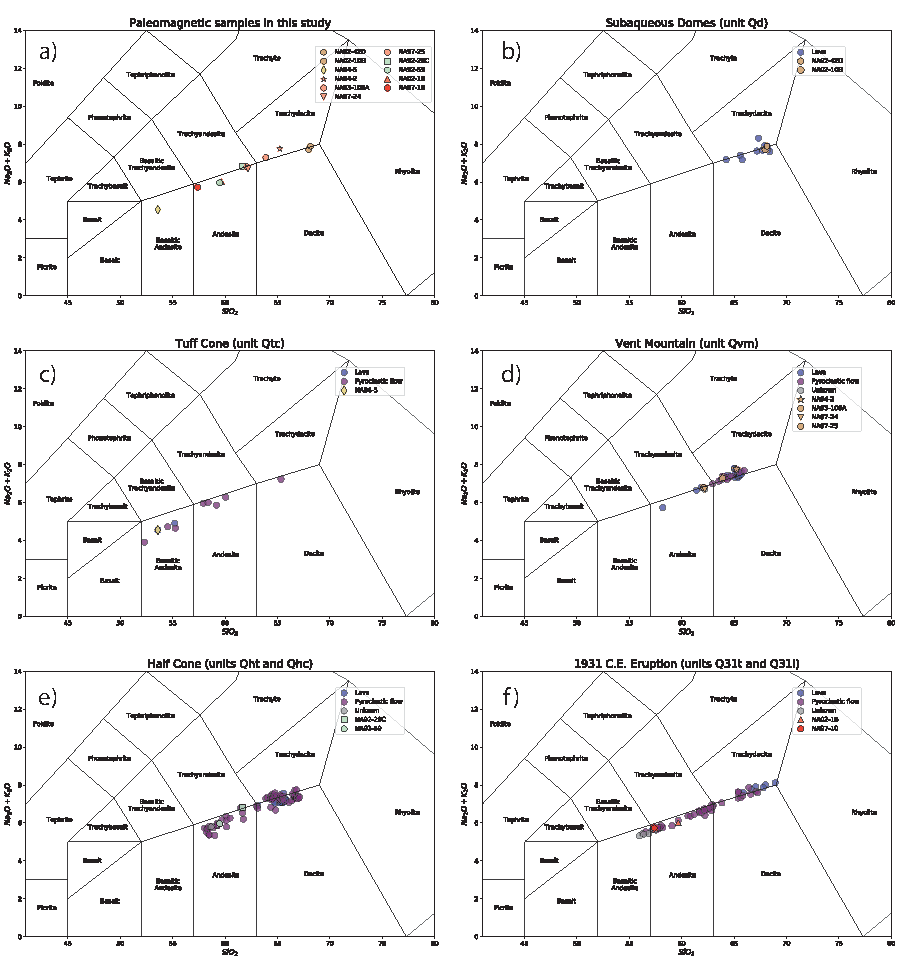
\includegraphics{../Figure/Geochem.pdf}
\caption{Total alkaline silica (TAS) plots for all Aniakchak units associated with this study. Plot a) includes all samples used in this study except for sample NA02-10F. Plots b to f show compilations of TAS measurements in Appendix Table B1 in \citeA{Bacon2014a} for all samples related to units of interests in this study. %Blue points are lava samples; red points are pyroclastic deposits; grey points represent samples with lithologies. R=rhyolite, O3=dacite, O2=Andesite, O1=basaltic andesite, Bs=tholeiitic basalt, Ba=alkaline basalt.
}
\label{TAS_plot}
\end{figure}

\section{Methods}
\subsection{Paleointensity Experiment}

Specimens were selected based on their visual and textural appearance for the paleointensity experiment (Figure \ref{Binocular_image}). The glassy textures shown in all specimens in Figure \ref{Binocular_image} here are indicative of rapid cooling, which tends to  %interpreted to be due to the formation of amorphous volcanic material during quenching. Such rapid cooling tend to 
promote the formation of single domain magnetic carriers that often succeed in paleointensity experiments \cite{Tauxe2004a}. Specimens chosen for the paleointensity experiment have glassy textures and have a minimum magnetic moment of $1.0E^{-7}$ Am$^{2}$. Specimens were wrapped in non-magnetic glass microfiber filters and glued inside 12 mm-diameter glass vials with potassium silicate. All glass vials were treated with a 600$^{\circ}$C heating in a zero-field to remove any remanent magnetization; vials used in the paleointensity experiment had a resulting magnetic moments smaller than $1.0E^{-10}$ Am$^{2}$. Between five and nine specimens were prepared for each sample (Table \ref{tab:samples}). 

\begin{figure}
\noindent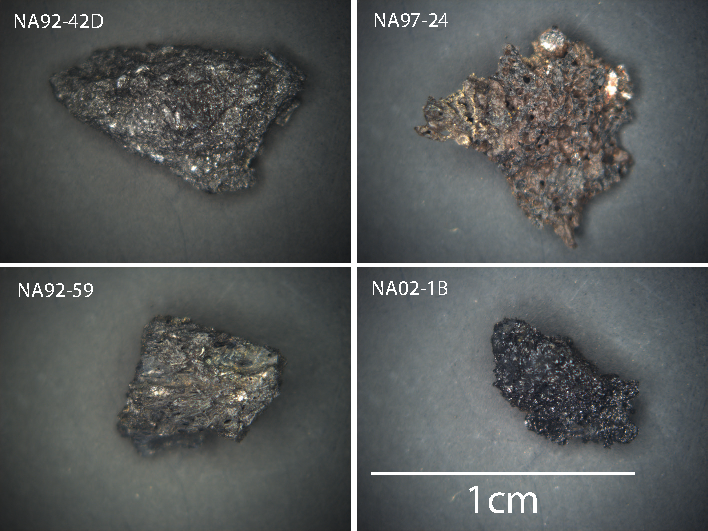
\includegraphics[width=35pc]{../Figure/Aniakchak_bino.pdf}
\caption{Binocular images of representative glassy volcanic materials that are sister specimens with those used for paleointensity experiments in this study. All images share the same scale as shown by the 1-centimeter scale bar in the image for sample NA02-1B. }
\label{Binocular_image}
\end{figure}

Paleointensity experiments were conducted at the paleomagnetic laboratory at Scripps Institution of Oceanography at the University of California San Diego. All experiments were conducted in a shielded room which had a background magnetic field less than 400 nanoTesla (nT). The IZZI-modified double heating protocol was used for the paleointensity experiment \cite{Yu2004a} using custom-built ovens. For zero-field heating steps the background magnetic field in the ovens was reduced to less than 5 nT. A laboratory field of 35 $\mu$T was applied during in-field heating steps along the Z-axis of the oven, parallel to the long axis of glass vials.  Specimens were treated up to $600^{\circ}$C or until at least 95\% of the natural remanent magnetization (NRM) was removed. Partial thermal remanent magnetization (pTRM) checks for alterations were applied at every other temperature step. NRM and pTRM measurements were performed using a 2G Cryogenic Magnetometer.

\subsection{Selection Criteria}
Data interpretation was performed using the Thellier GUI Auto Interpreter \cite{Shaar2013a}, part of the PmagPy software package \cite{Tauxe2016a}, using the CCRIT  selection criteria \cite{Cromwell2015b}. CCRIT was designed to limit the selected specimen results to be those containing only a single directional magnetic component and near-linear slopes in NRM/TRM Arai plots \cite{Arai1963a}. This criteria has been useful in filtering out non-ideal specimens, such as those with poor Arai behavior and those producing poor within-sample paleointensity dispersion. Specimen- and sample-level requirements of CCRIT are listed in Table \ref{tab:criteria}, and brief descriptions are provided below (more detailed explanations of each criterium are presented in \citeA{Paterson2014a}. $\beta$ is the standard deviation of the slope of selected data points normalized by the absolute value of the slope. $SCAT$ is a Boolean based on the value of $\beta$ and evaluates the degree of scatter of the selected data points about the best fit slope. Here the threshold of $\beta$ is set at 0.1. $FRAC$ measures the fraction of the NRM used in calculating the best fit line. \textit{Gap Max} sets the maximum gap between two consecutive NRM/TRM points on Arai plot. MAD is the maximum angle of deviation representing the scatter of selected through demagnetization procedures about the unanchored best fit line. DANG measures the angle between the best fit line and the line determined by the center of mass of the selected data points and the origin. $|\vec{k}|$ is the absolute value of the degree of curvature of selected data points on Arai plots, put forward by \citeA{Paterson2011a}. A larger value of $|\vec{k}|$ indicates a more curved Arai plot. \textit{N} is the minimum number of accepted specimens to calculate the sample-mean intensity. $B_{\sigma}$ is the maximum accepted one-sigma standard deviation of sample-mean intensity, and $B_{\sigma} \%$ is the maximum accepted percentage of $B_{\sigma}$ relative to the sample-mean intensity; successful samples may not exceed both $B_{\sigma}$ and $B_{\sigma} \%$ .

\section{Results and Discussion}

A total of 36 out of 89 specimens passed the specimen-level CCRIT selection criteria. 6 out of 13 samples passed the sample-level selection criteria and yielded high-quality absolute paleointensity results. Estimated paleointensity results from all accepted samples are listed in Table \ref{tab:samples} and plotted as black symbols in Figure \ref{VADM_comparisons}. Specimen-level paleointensity estimates and statistics for accepted samples are listed in Table \ref{tab:specimens}. All sample- and specimen-level experimental results are archived in the MagIC database at \url{https://earthref.org/MagIC/19326}. Successful samples have a mean paleointensity value of 58.8 $\mu$T with a standard deviation of 5.6 $\mu$T, which corresponds to a mean virtual axial dipole moment (VADM) of 86.3 $\times 10^{21}$ Am$^{2}$ (ZAm$^{2}$) with a standard deviation of 4.93 ZAm$^{2}$. The range of paleointensity values for the successful samples ranged from 49.5 to 68.0 $\mu$T, corresponding to VADM values that range from 63.7 to 99.8 ZAm$^{2}$ (Figure \ref{VADM_comparisons}).

\begin{figure}
\noindent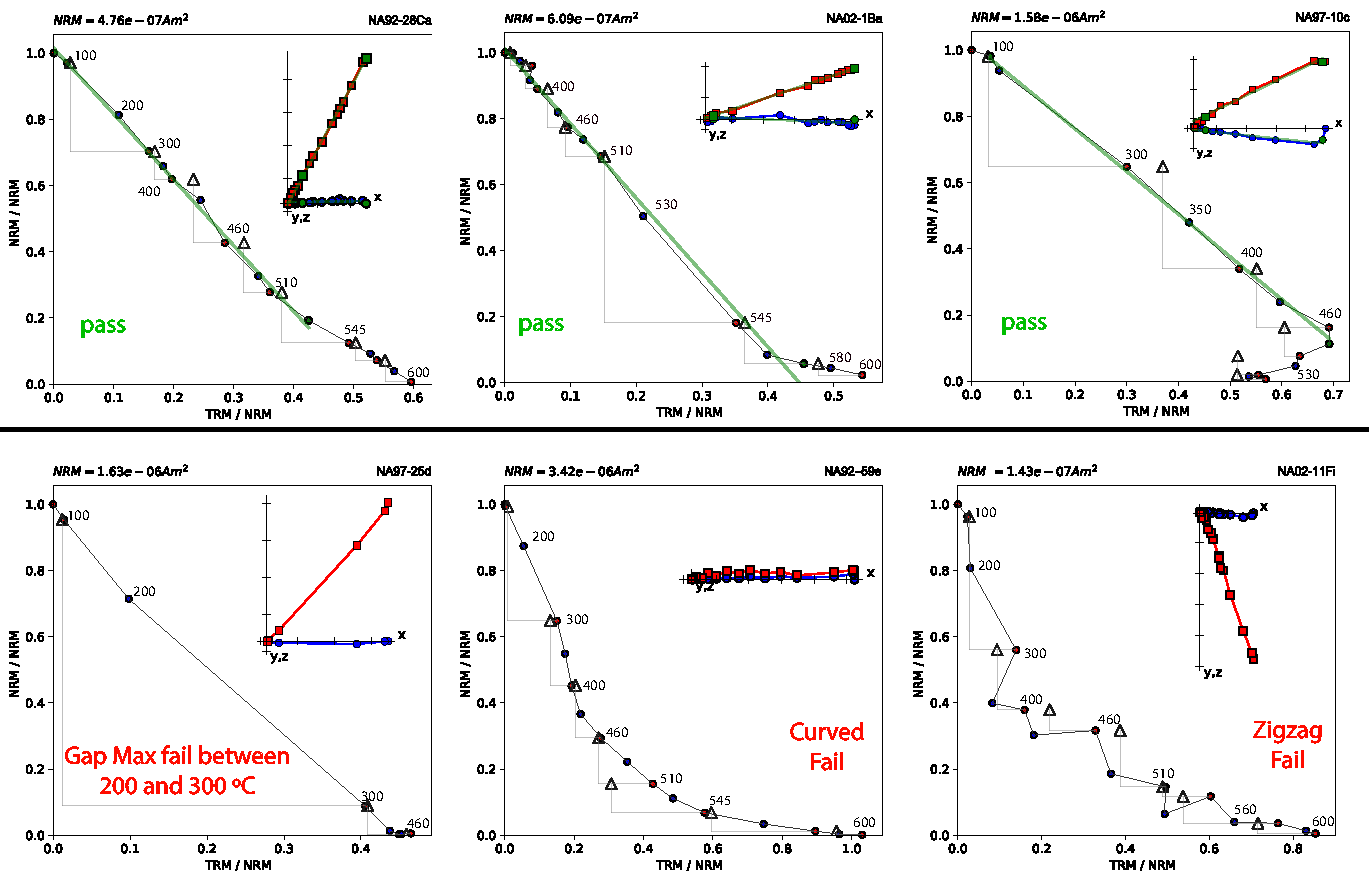
\includegraphics[width=30pc]{../Figure/IZZI_results_revision.pdf}
\caption{Representative specimen paleointensity Arai plots, showing normalized thermal remanent magnetization acquired during in-field heating steps plotted against normalized natural remanent magnetization removed during zero-field steps. In the Arai plots, temperature values are listed in degree Celsius, pTRM checks are shown as triangles, zero-field/in-field temperature steps are shown as red dots, in-field/zero-field steps are shown in blue. The green line is the least-squares component fit for selected temperature steps for specimens that pass the selection criteria. Inset orthogonal vector demagnetization diagrams (in specimen coordinates) show that the specimens have dominantly single component remanent magnetizations. Figures in the top row show typical paleointensity behavior of specimens with dominantly straight slope of NRM/TRM that pass the CCRIT selection criteria \cite{Cromwell2015b}; the bottom row shows typical behavior of specimens that fail the selection criteria.
}
\label{IZZI_results}
\end{figure}

Representative specimen results from the IZZI paleointensity experiment are shown in Figure \ref{IZZI_results} as NRM/TRM paleointensity plots and orthogonal demagnetization plots. Specimens in samples that passed CCRIT exhibit linear ratios between TRM acquired during in-field steps and NRM lost during associated zero-field steps, with reproducible pTRM checks (Figure \ref{IZZI_results}). Specimens from the same sample that pass the paleointensity result selection generally have consistent behaviors, likely associated with their close mineralogy assemblages. The majority of accepted specimens show single-component orthogonal demagnetization plots (Figure \ref{IZZI_results}), consistent with the interpretation that they have retained primary NRMs during cooling after eruption and have acquired minimum secondary overprints. 

Specimens that did not pass CCRIT (Figure \ref{IZZI_results}) selection were rejected for displaying non-linear TRM/NRM behavior over the course of the heating experiment. For example, specimen NA02-11Fi and NA92-59e (Figure \ref{IZZI_results}) exhibit zigzagging and sagging Arai plot with failed pTRM checks beginning at 300$^{\circ}$C and 510$^{\circ}$C respectively. This is likely due to the contribution of vortex state or multi-domain (MD) magnetic grains within the specimens. Because vortex state and MD grains often unblock differently between in-field and zero-field steps \cite{Tauxe2004a, Yu2004a}, the alternating steps of in-field/zero-field (IZ) and zero-field/in-field (ZI) IZZI experimental protocol results in zigzagging or sagging of the Arai plot. Specimen NA97-25d has a linear Arai plot, but it fails the Gap Max criterion because of the great loss of NRM intensity between temperature steps 200$^{\circ}$C and 300$^{\circ}$C. In addition, the majority of the remanence in this specimen was removed after the 300$^{\circ}$C heating step, indicating that the dominant magnetic carrier within the specimen is not likely stochiometric single-domain magnetite and may be prone to secondary overprint. %Therefore such paleointensity result is excluded from our further analyses. 

\begin{figure}
\centering
\noindent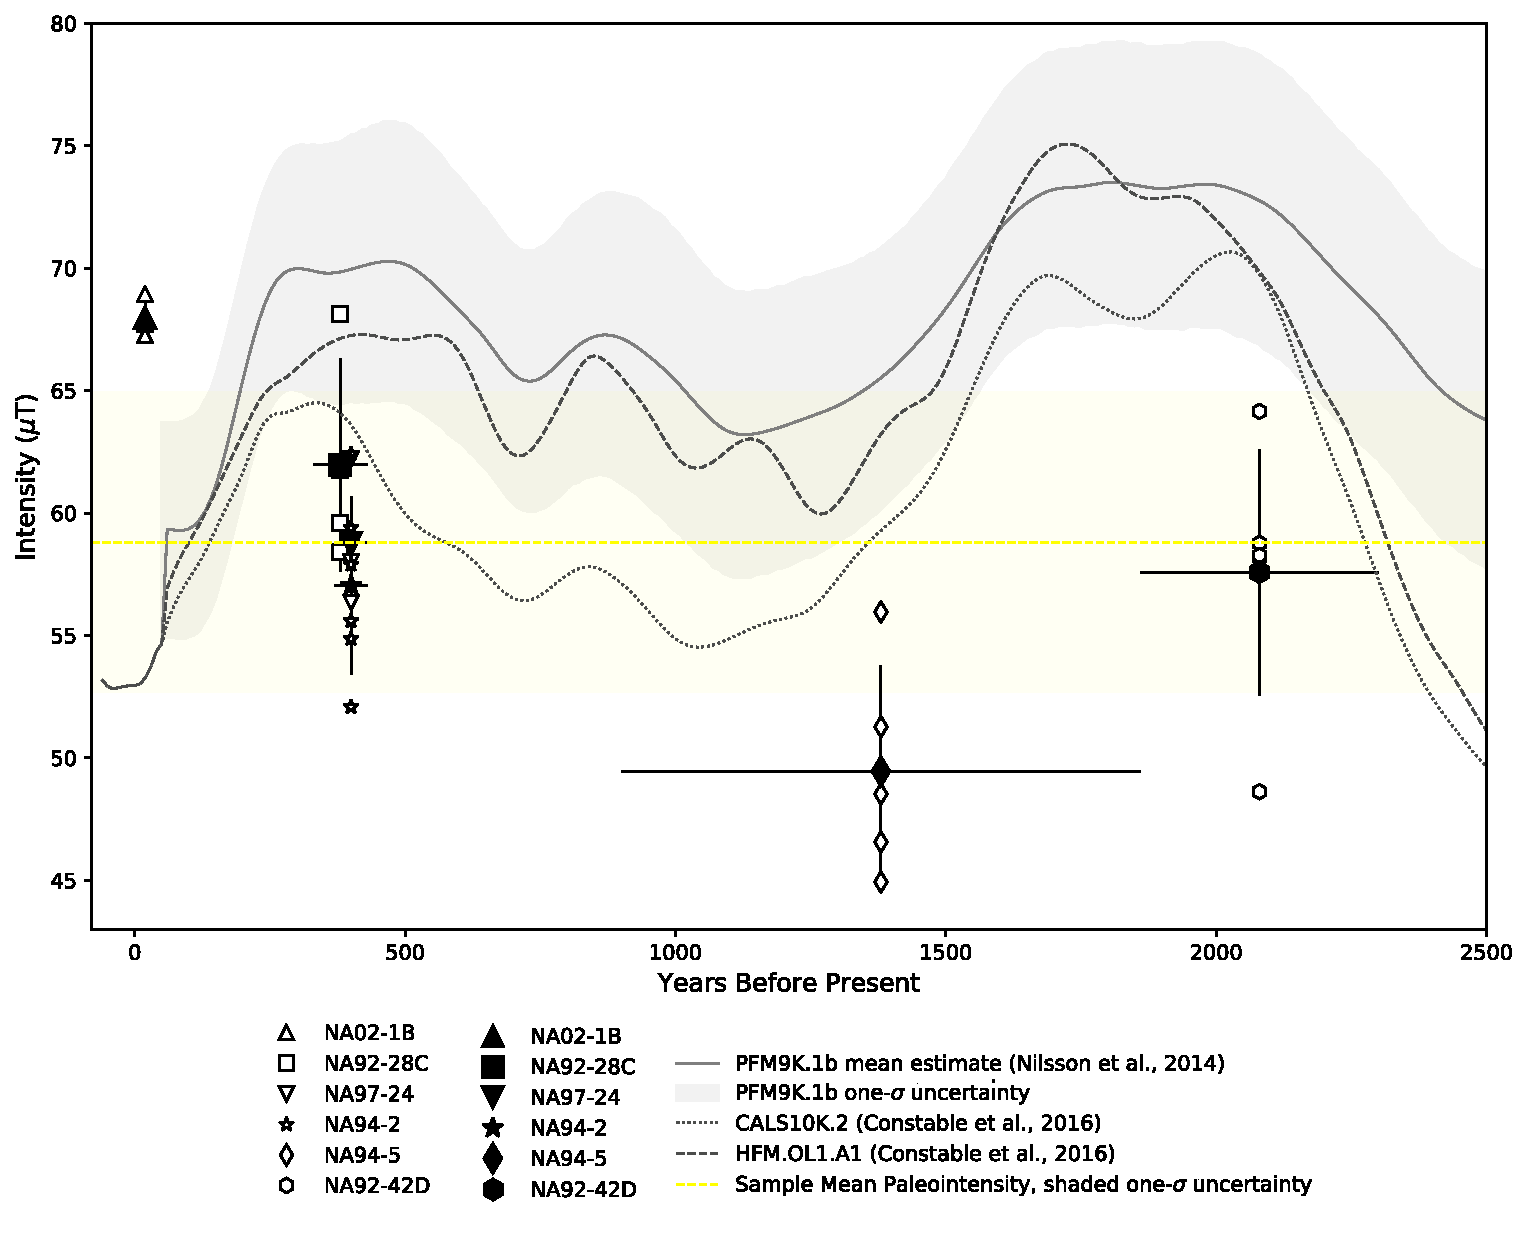
\includegraphics[width=30pc]{../Figure/VADM_comparison_revision_092321.pdf}
\caption{Summary of absolute paleointensity results from Aniakchak volcano with respect to predicted paleointensity values at Aniakchak volcano from global geomagnetic field models PFM9k.1b \cite{Nilsson2014a}, CALS10k.2 \cite{Constable2016a}, and HFM.OL1.A1 \cite{Constable2016a}. The 1$\sigma$-uncertainty for model PFM9k.1b is shown as the grey area. Individual specimen paleointensity estimates (open symbols), sample-level average paleointensity results (closed symbols), together with one standard deviation uncertainties are plotted with respect to their estimated ages with uncertainties. Dashed yellow line and yellow rectangular area represents the mean paleointensity value of all samples (58.8 $\mu$T) and one standard deviation uncertainty. 1950 C.E. is used as zero years before present.}
\label{VADM_comparisons}
\end{figure}

Figure \ref{VADM_comparisons} summarizes individual specimen paleointensity results, sample-mean paleointensity results with one standard deviations, and locality-mean value of all successful samples, 58.8 $\mu$T. Shown for comparison are the mean of the %present-day geomagnetic field intensity at Aniakchak volcano, and 
predicted surface intensities from global geomagnetic field model estimates at Aniakchak volcano for the last 2,500 yrs B.P. from models PFM9K.1b \cite{Nilsson2014a}, CALS10k.2 \cite{Constable2016a}, and HFMOL1.A1 \cite{Constable2016a}. Specimens from samples that passed the CCRIT selection criteria generally yield consistent specimen-level paleointensity estimates. The overall sample-mean paleointensity estimates show a similar trend in field intensity as predicted by the geomagnetic field models, although the absolute paleointensity values of the samples tends to be lower than that of the models (Figure \ref{VADM_comparisons}). The sample and model intensities follow a high-low-high trend from \textit{ca.} 2,300 to the present; they tend to peak between about 1,600 and 2,000 yrs B.P., decline to a low at about 1,300 yrs B.P., and peak again between about 300 and 500 yrs B.P.  . 

The mean paleointensity estimate from sample NA92-42D which is from the subaqueous domes (unit Qd), is lower than the predicted values from the geomagnetic field models at \textit{ca.} 2,100 yrs B.P. However, given its estimated age range between 1,860 yrs B.P. and 2,300 yrs B.P., an interpretation could be allowed that this sample was emplaced close to 2,300 yrs B.P. during the widespread pumice fall that was synchronous with or predates the emplacement of the subaqueous domes \cite{Bacon2014a}. %the catastrophic draining of the ancestral caldera lake of Aniakchak. Such interpretation favors that the subaqueous domes (unit Qd) were active nearer to the older end of the $^{14}$C age constraint of \textit{ca.} 2,300 yrs B.P.
If sample NA92-42D was emplaced close to 2,300 yrs B.P., its paleointensity value would be consistent with those  predicted by models CALS10k.2 and HFMOL1.A1 and nearly within uncertainty of model PFM9K.1b  (Figure \ref{VADM_comparisons}). 

Sample NA94-5 from Tuff Cone (unit Qtc) has a mean paleointensity estimate lower than what is predicted by all three geomagnetic field models (Figure \ref{VADM_comparisons}). This sample has a broad estimated age range between 900 yrs B.P. and 1860 yrs B.P. If the age of this sample is closer to the minimum age estimate (as may be indicated by geochemical data, see "Stratigraphy and Age Constraints" section) then the range of paleointensity values of sample NA94-5 could be more consistent with the relatively low intensity values predicted by the three geomagnetic field models at about 1,100 yrs. B.P. If this was the case, the paleointensity of sample NA94-5 would be consistent with the predicted decreasing trend in geomagnetic field intensity at Aniakchak volcano since the high between about 1,600 and 2,000 yrs B.P., although the estimated absolute field intensity would underestimate that predicted by the field models. 

Samples NA94-2 and NA97-24 from Vent Mountain (unit Qvm), and sample NA92-28C from Half Cone (unit Qht) have similar estimated ages of 400$\pm$30 and 380$\pm$50 yrs B.P., respectively, and have indistinguishable estimated paleointensity values within the calculated uncertainty.   (Table\ref{tab:samples}; Figure \ref{VADM_comparisons}). Despite having equivalent paleointensity estimates, the mean value of the individual samples vary with respect to the predicted intensity of the geomagnetic field models. Samples NA94-2 and NA97-24 have lower estimated intensities than all three field models, while the uncertainty bounds of sample NA92-28C are consistent with model CALS10k.2 and within the uncertainty of model PFM9K.1b. The paleointensity of samples NA94-2, NA97-24, and NA92-28C follow the predicted increasing trend in geomagnetic field intensity at Aniakchak volcano since about 1,100 yrs B.P., although the absolute field intensity values from the samples are generally lower than those predicted by the field models.


%Considering their estimated age range, the paleointensity estimates from these samples are consistent with the predicted values of model CALS10k.2 at the time of Vent Mountain and Half Cone eruptions (Figure \ref{VADM_comparisons}). 
%The relatively higher paleointensity estimates from these samples are consistent with the increasing trend over several hundred years from the time Tuff Cone eruption to Vent Mountain and Half Cone eruptions. 

Sample NA02-1B from the 1931 C.E. tephra (unit Q3t) has a mean paleointensity estimate of 68.0 $\mu$T, about 15 $\mu$T (25\%) higher than the historical field strength at Aniakchak volcano in 1931 C.E. (53.2 $\mu$T; estimated from IGRF12 using igrf.py, included as part of the PmagPy software package;\cite{Tauxe2016a}) and greater than the predicted intensity from the geomagnetic field models (Table \ref{tab:samples}; Figure \ref{VADM_comparisons}). The substantial overestimate of the historical field strength warrants additional consideration of the experimental results for sample NA01-1B together with sample NA97-10, which was also emplaced during the 1931 C.E. eruption (part of the 1931 C.E. lava flow unit, Q3l). Arai plots of specimens from sample NA02-1B show hints of double-slope behavior that could be the result of unrecognized thermochemical alterations or post-emplacement heating, which could reduce the accuracy of the paleointensity interpretations from specimens that pass CCRIT (top left plot in Figure \ref{IZZI_results}; \citeA{Bowles2015b}). The double-slope behaviors in these specimens include a low temperature component between 0–300$^{\circ}$C and a higher temperature component between 350–560$^{\circ}$C. After 560$^{\circ}$C the specimens show signs of alteration as evidenced by failed pTRM checks (Figure \ref{IZZI_results}). These specimens pass the CCRIT selection criteria despite observed non-linearity in the Arai plots, and yield consistent inter-sample paleointensity results (Figure \ref{IZZI_results}; Table \ref{tab:samples} and \ref{tab:specimens}). Nevertheless, the possibility remains that the presence of MD grains or post-emplacement alterations could have led to erroneous paleointensity estimates.   

Two specimens from sample NA97-10 pass the specimen-level CCRIT selection criteria and have estimated paleointensity values of 38.7 $\mu$T and 49.1 $\mu$T (Tables \ref{tab:samples} and \ref{tab:specimens}). However, sample NA97-10 failed the CCRIT sample-level criteria because a minimum of three specimens is required. The two successful specimens have linear Arai plots up to 460$^{\circ}$C, after which they show signs of alteration as evidenced by failed pTRM checks (top right plot in Figure \ref{IZZI_results}). Like the specimens from NA02-1B, the Arai plots of specimens from NA97-10 show hints of double-slope behavior at lower temperatures, as well as directional overprints in the Zijderveld diagrams. The successful specimen intensity values are about 4 to 15 $\mu$T lower than the historical field strength at Aniakchak volcano (53.2 $\mu$T) and at least 19 $\mu$T lower than the mean intensity for sample NA02-1B (68.0 $\mu$T). If the successful specimens from both 1931 C.E. samples were combined, the resulting mean paleointensity would be 58.3$\pm$13.7 $\mu$T and would have encompassed the historical field strength, although the resulting estimate would have failed the CCRIT $B_{\sigma}$ and $B_{\sigma} \%$ sample-level criteria.

\begin{figure}
\centering
\noindent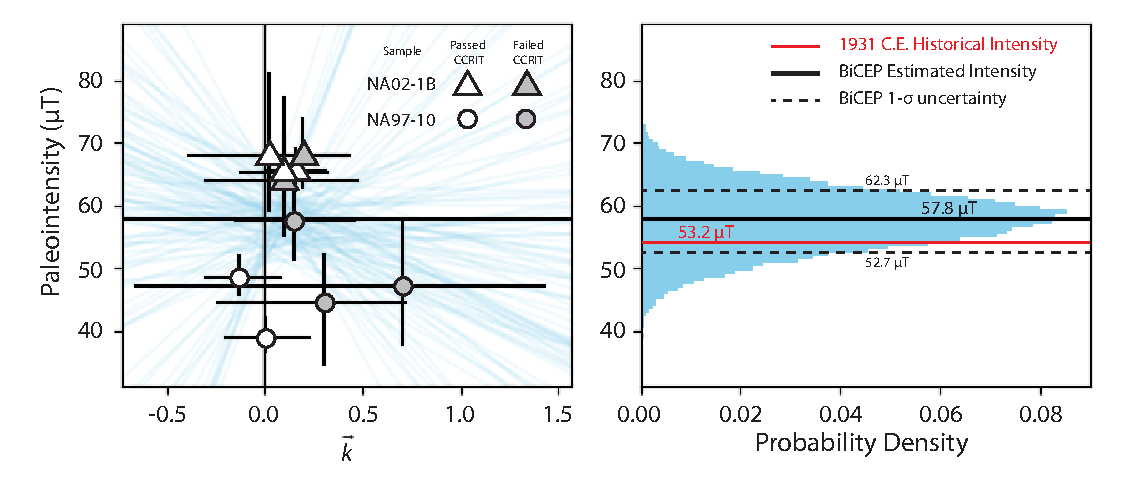
\includegraphics[width=35pc]{../Figure/BiCEP_1931_all_092421.pdf}
\caption{Estimated paleointensity results of the 1931 C.E. eruption from the Bias Corrected Estimation of Paleointensity (BiCEP) method \cite{Cych2021a}. Left plot, estimated range of individual specimen paleointensity estimates relative to the estimated $\vec{k}$; right plot, resulting estimate of 1931 C.E. field intensity and probability distribution.}
\label{bicep_1931}
\end{figure}

We apply the Bias Corrected Estimation of Paleointensity (BiCEP) method of \citeA{Cych2021a} as a different means of estimating the paleointensity and uncertainty from the 1931 C.E. samples. BiCEP is a Bayesian method which accounts for bias in paleointensity estimates of specimens, effectively weighting the paleointensity of different specimens using the curvature of the Arai plot as a metric of nonlinearity (where linearity is measured by the $\vec{k}$ statistic) and a predictor of bias \cite{Cych2021a}. Specimen paleointensity and bias are estimated using a range of selected temperature steps in the Arai plot. For the BiCEP calculation, we provided temperature steps for all specimens from samples NA02-1B and NA97-10, including those that failed the CCRIT selection criteria (Table \ref{tab:bicep}). For the specimens that passed CCRIT, we used the temperature steps from the Thellier-GUI estimation (Table \ref{tab:specimens}). For the specimens that failed CCRIT we provided the temperature steps that represented the characteristic NRM/TRM of the paleointensity experiment, excluding low-temperature steps that deviate from the characteristic remanent magnetization direction on the Zijderveld plots, and high-temperature steps where thermochemical alteration occurred as evidenced by failed pTRM checks in the Arai plot. 

The BiCEP estimation using all specimens from samples NA02-1B and NA97-10 generated ``B-Grade" results \cite{Cych2021a}, which are shown in Figure \ref{bicep_1931}. The range of individual specimen paleointensity estimates relative to the range of estimated $\vec{k}$ is shown on the left plot of Figure \ref{bicep_1931}. The distribution and range of estimates on the plot is typical to the BiCEP calculation when the specimen-level experimental results have a range of quality and linearity in their Arai plot. The resulting probability distribution of estimated paleointensities is shown on the right plot of Figure \ref{bicep_1931}. The median paleointensity value from the probability distribution was 57.8 $\mu$T, about 4.5$\mu$T higher than the 1931 C.E. historical field intensity (Figure \ref{bicep_1931}). The calculated 1-$\sigma$ uncertainty range from BiCEP was 52.7$\mu$T and 62.3$\mu$T. The resulting paleointensity estimate from BiCEP is within the 1-$\sigma$ uncertainty range of the historical field strength for 1931 C.E. The BiCEP method provides a reasonable estimate and associated uncertainty of the 1931 C.E. field intensity at Aniakchak volcano based on the experimental results from the available samples. The inter-sample variability between the 1931 C.E. samples indicates that there may be rock magnetic, mineralogical, and (or) post-emplacement effects  that affected the viability of the paleointensity experiment, warranting further investigation of these samples and additional sample collection.


\section{Conclusion}
In this study we report high-quality paleointensity results for the past 2,300 years from rapidly cooled, glassy volcanic material from Aniakchak volcano, Alaska, USA. Six samples pass the CCRIT selection criteria and provide paleointensity estimates. These new paleointensity results are a valuable contribution to the mid- to high-northern latitude paleomagnetic dataset for North America. Although our sample-mean paleointensities are generally lower than predicted model intensities, paleointensity results for five samples are generally consistent with predicted variability in field strengths from global geomagnetic field models, considering age and experimental uncertainties. One sample for the historical 1931 C.E. eruption passed the CCRIT selection criteria and had robust inter-specimen consistency. However it yielded a paleointensity result about 15 $\mu$T higher than the historical field strength. Further analyses using a Bayesian estimation method of specimens from this sample and another sample from the 1931 C.E. eruption yielded a probability estimate with 1-$\sigma$ uncertainty that is consistent with the historical field strength. Further investigation of samples from the 1931 C.E. eruption is warranted to investigate potential rock magnetic, mineralogical, and (or) post-emplacement effects on the paleointensity results. Overall, the paleointensity results from Aniakchak volcano help provide new spatial and temporal coverage for future geomagnetic field models. Additional sampling of glassy volcanic materials paired with more precise age controls in future studies at Aniakchak volcano and other volcanoes along the Alaska-Aleutian arc will further constrain estimates of geomagnetic field behavior in North America.



\begin{landscape}
\footnotesize
\LTcapwidth=1.5\textwidth
\begin{longtable}{lcccccccccl}
\caption{Table of location information, field observations, estimated ages, absolute paleointensity results, and calculated VADM values for all samples. \textit{Lat} and \textit{Lon} are degrees latitude (north) and longitude (east) based on datum NAD83. \textit{Age} is interpreted sample age (years before calendar year 1950 C.E.) and age uncertainty (years). \textit{Unit} is the map unit from Figure \ref{Geologic_map}. $nn$ is number of accepted specimens for successful samples, and $n$ is total specimens measured. $B_{F}$ is the estimated ancient field strength in $\mu$T, $B_{F} \sigma$ is the standard deviation of $B_{F}$. VADM (virtual axial dipole moment) and VADM $\sigma$ values are in Am$^{2}$. \textit{Sample Location and Description} are descriptions of the field locality and physical sample.}\\

\hline
	Sample	&	Lat	&	Lon	&	Age 	&	Unit	&	$nn/n$	&	$B_{F}$	&	$B_{F} \sigma$	&	VADM	&	VADM $\sigma$		&	Sample Location and Description
\\
\hline
NA92-42D	&	56.9026	&	-158.2243	&	1,860–2,300	&	Qd	&	6/7	&	57.6	&	5.02	&	8.45E+22	&	7.37E+21	& 1931 Main Crater, west wall; \\								
	&		&		&		&		&		&		&		&		&		&   pre-Half Cone, dense, gray, sparsely porphyritic lava flow, platy jointing \\								
NA02-10G	&	56.9015	&	-158.2244	&	1,860–2,300	&	Qd	&	--/7	&	--	&	--	&	--	&		--	&	1931 Main Crater west wall;	\\					
	&		&		&		&		&		&		&		&		&		&		dense, gray lava flow with platy jointing high in west 1931 crater wall	\\					
NA94-5	&	56.8951	&	-158.0882	&	900–1,860	&	Qtc?	&	5/9	&	49.5	&	4.34	&	7.26E+22	&	6.37E+21	&	Lowest flow terrace below big maar;	\\						
	&		&		&		&		&		&		&		&		&		&	older lava flow near The Gates; possible Windy Cone source \\							
NA94-2	&	56.8793	&	-158.1358	&	400$\pm$30	&	Qvm	&	6/6	&	57.0	&	3.65	&	8.37E+22	&	5.36E+21	&	New Cone rim, southeast flank of Vent Mountain;	\\						
	&		&		&		&		&		&		&		&		&		& dark brown, scoriaceous, porphyritic pumice\\								
NA97-24	&	56.88	&	-158.134	&	400$\pm$30	&	Qvm	&	6/7	&	58.8	&	1.91	&	8.63E+22	&	2.80E+21	&	East rim New Cone crater;\\							
	&		&		&		&		&		&		&		&		&		&New Cone agglutinate\\								
NA97-25	&	56.8859	&	-158.1248	&	400$\pm$30	&	Qvm	&	--/6	&	--	&	--	&	--	&		--	& Alluvial flat east of Vent Mountain;	\\						
	&		&		&		&		&		&		&		&		&		&Vent Mountain lava, possibly related to New Cone	\\							
NA93-100A	&	56.8939	&	-158.1294	&	840–900	&	Qvm	&	2/7	&	--	&	--	&	--	&		--	&	East base of Vent Mountain;	\\					
	&		&		&		&		&		&		&		&		&		&Vent Mountain lava younger than tuff cones, at base of tephra section \\								
NA92-28C	&	56.9076	&	-158.2019	&	380$\pm$50	&	Qht	&	4/6	&	62.0	&	4.34	&	9.09E+22	&	6.37E+21	& 1931 Main Crater wall;	\\							
	&		&		&		&		&		&		&		&		&				& Half Cone agglutinate	\\					
NA92-59	&	56.895	&	-158.1686	&	380$\pm$50	&	Qht	&	2/6	&		--	&	--	&	--	&		--	&	North base Vent Mountain;	\\				
	&		&		&		&		&		&		&		&		&				& Half Cone agglutinate	\\					
NA02-10F	&	56.9015	&	-158.2244	&	380$\pm$50	&	Qht?	&	--/9	&	--	&	--	&	--	&		--	&	1931 Main Crater west wall;	\\					
	&		&		&		&		&		&		&		&		&		&		black agglutinate half cone? 	\\					
NA02-11F	&	56.9066	&	-158.2132	&	$>$ 840$\pm$40	&	Qhc?	&	--/9	&		--	&	--	&	--	&		--	&	1931 Main Crater north wall;	\\				
	&		&		&		&		&		&		&		&		&				&welded volcaniclastic	\\					
NA02-1B	&	56.8893	&	-158.191	&	1931 C.E.	&	Q31t?	&	3/5	&	68.0	&	0.88	&	9.98E+22	&	1.29E+21		&	Between Blocky Cone and the base of Vent Mountain;	\\					
	&		&		&		&		&		&		&		&		&				& 1931 scoria\\						
NA97-10	&	56.908	&	-158.21	&	1931 C.E.	&	Q31l	&	2/5	&	--	&	--	&	--	&		--	&	1931 Main Crater floor near base of north wall; \\						
	&		&		&		&		&		&		&		&		&				&	1931 spatter-fed lava flow	\\						
\hline																										


%\end{tabular}
\label{tab:samples}
\end{longtable}
%\end{center}
\end{landscape}

\begin{table}
\caption{Specimen- and sample-level criteria for the CCRIT \protect\cite{Cromwell2015a} selection method (\textit{SCAT} criterion uses a $\beta_{threshold}$ value of 0.1). Refer to the ``Selection Criteria" section or \protect\citeA{Paterson2014a} for descriptions of each statistic.} 
\begin{tabular}{ccccccc|ccc}
\hline
\multicolumn{10}{c}{CCRIT Paleointensity Selection Criteria}\\ 
\hline
\multicolumn{7}{c} {\underline{\textit{Specimen}}}
&
\multicolumn{3}{c} {\underline{\textit{Sample}}}\\
\textit{SCAT}&\textit{FRAC}&\textit{Gap Max}&$\beta$&\textit{MAD$_{free}$}&\textit{DANG}&$|\vec{k}|$&\textit{N}&$B_{\sigma}$&$B_{\sigma}$~$\%$\\
\hline
PASS&$\ge$ 0.78&$\le$ 0.60&$\le$ 0.10&$\le$ 5.0$^{\circ}$&$\le$ 10.0$^{\circ}$&$\le$ 0.164&$\ge3$&$\le$ 4 $\mu$T&$\le$ 10~\%\\
\hline

\end{tabular}
\label{tab:criteria}
\end{table}

\begin{landscape}
\footnotesize
\LTcapwidth=1.5\textwidth
\begin{longtable}{llcccccccccccc}
\caption{Summary table of specimen-level paleointensity experiment results. Paleointensity results and selection criteria statistics are listed for specimens that passed the CCRIT selection criteria. Specimen and Sample are paleomagnetic specimens and their respective samples. $B_{F}$ is the measured intensity in microTesla, $T_{low}$ and $T_{high}$ are lower and upper temperature bounds (degrees Celcius) used to calculate intensity, and $n$ and $n_{pTRM}$ are the number of temperature steps and pTRM checks used in that same calculation. \textit{SCAT}, \textit{FRAC}, \textit{Gap Max}, $\beta$, $MAD_{free}$, \textit{DANG}, and $|\vec{k}|$ are statistics used to determine specimen reliability. See “Selection Criteria” section for a description of all statistics, and Table \ref{tab:criteria} for selection criteria.}\\

\hline
Specimen	&	Sample	&	$B_{F}$	&	$T_{low}$	&	$T_{high}$	&	$n$	&	$n_{pTRM}$	&	\textit{SCAT}	&	\textit{FRAC}	&	\textit{Gap Max}&	$\beta$	&	$MAD_{free}$	&	\textit{DANG}	&	$|\vec{k}|$
 \\
\hline
NA92-42Da	&	NA92-42D	&	58.76	&	0	&	400	&	6	&	2	&	PASS	&	0.92	&	0.46	&	0.08	&	3.6	&	1.56	&	-0.02	\\
NA92-42Db	&	NA92-42D	&	58.16	&	100	&	400	&	5	&	2	&	PASS	&	0.88	&	0.52	&	0.06	&	2.02	&	2.37	&	-0.08	\\
NA92-42Dc	&	NA92-42D	&	58.27	&	100	&	400	&	5	&	2	&	PASS	&	0.89	&	0.51	&	0.05	&	2.99	&	3.01	&	0	\\
NA92-42Dd	&	NA92-42D	&	64.15	&	0	&	430	&	7	&	2	&	PASS	&	0.95	&	0.48	&	0.04	&	1.76	&	1.6	&	0.04	\\
NA92-42De	&	NA92-42D	&	57.53	&	0	&	400	&	6	&	2	&	PASS	&	0.92	&	0.46	&	0.05	&	2.24	&	2.39	&	0.08	\\
NA92-42Df	&	NA92-42D	&	48.62	&	100	&	460	&	7	&	3	&	PASS	&	0.92	&	0.55	&	0.04	&	3.92	&	2.37	&	-0.1	\\
NA92-42Dg	&	NA92-42D	&	–	&	–	&	–	&	–	&	–	&	–	&	–	&	–	&	–	&	–	&	–	&	–	\\
NA02-10Ga	&	NA02-10G	&	–	&	–	&	–	&	–	&	–	&	–	&	–	&	–	&	–	&	–	&	–	&	–	\\
NA02-10Gb	&	NA02-10G	&	–	&	–	&	–	&	–	&	–	&	–	&	–	&	–	&	–	&	–	&	–	&	–	\\
NA02-10Gc	&	NA02-10G	&	–	&	–	&	–	&	–	&	–	&	–	&	–	&	–	&	–	&	–	&	–	&	–	\\
NA02-10Gd	&	NA02-10G	&	–	&	–	&	–	&	–	&	–	&	–	&	–	&	–	&	–	&	–	&	–	&	–	\\
NA02-10Ge	&	NA02-10G	&	–	&	–	&	–	&	–	&	–	&	–	&	–	&	–	&	–	&	–	&	–	&	–	\\
NA02-10Gf	&	NA02-10G	&	–	&	–	&	–	&	–	&	–	&	–	&	–	&	–	&	–	&	–	&	–	&	–	\\
NA02-10Gg	&	NA02-10G	&	–	&	–	&	–	&	–	&	–	&	–	&	–	&	–	&	–	&	–	&	–	&	–	\\
NA94-5a	&	NA94-5	&	–	&	–	&	–	&	–	&	–	&	–	&	–	&	–	&	–	&	–	&	–	&	–	\\
NA94-5b	&	NA94-5	&	48.53	&	0	&	430	&	7	&	2	&	PASS	&	0.81	&	0.37	&	0.05	&	4.88	&	4.88	&	0.16	\\
NA94-5c	&	NA94-5	&	46.57	&	0	&	430	&	7	&	2	&	PASS	&	0.79	&	0.34	&	0.06	&	3.56	&	1.39	&	0	\\
NA94-5d	&	NA94-5	&	–	&	–	&	–	&	–	&	–	&	–	&	–	&	–	&	–	&	–	&	–	&	–	\\
NA94-5e	&	NA94-5	&	–	&	–	&	–	&	–	&	–	&	–	&	–	&	–	&	–	&	–	&	–	&	–	\\
NA94-5f	&	NA94-5	&	51.27	&	0	&	430	&	7	&	2	&	PASS	&	0.85	&	0.35	&	0.06	&	3.17	&	2.29	&	0.12	\\
NA94-5g	&	NA94-5	&	–	&	–	&	–	&	–	&	–	&	–	&	–	&	–	&	–	&	–	&	–	&	–	\\
NA94-5h	&	NA94-5	&	55.96	&	200	&	560	&	11	&	5	&	PASS	&	0.89	&	0.21	&	0.04	&	4.96	&	1.22	&	0	\\
NA94-5i	&	NA94-5	&	44.93	&	200	&	580	&	12	&	6	&	PASS	&	0.84	&	0.14	&	0.04	&	2.86	&	0.97	&	-0.04	\\
NA94-2a	&	NA94-2	&	55.59	&	100	&	460	&	7	&	3	&	PASS	&	0.95	&	0.59	&	0.02	&	1.86	&	0.81	&	0	\\
NA94-2b	&	NA94-2	&	57.9	&	0	&	490	&	9	&	3	&	PASS	&	0.96	&	0.52	&	0.05	&	2.89	&	0.93	&	0.15	\\
NA94-2c	&	NA94-2	&	59.4	&	0	&	510	&	10	&	4	&	PASS	&	0.99	&	0.54	&	0.03	&	1.54	&	0.79	&	0.16	\\
NA94-2d	&	NA94-2	&	54.87	&	0	&	460	&	8	&	3	&	PASS	&	0.97	&	0.46	&	0.04	&	1.44	&	1.1	&	-0.04	\\
NA94-2e	&	NA94-2	&	52.08	&	100	&	460	&	7	&	3	&	PASS	&	0.95	&	0.59	&	0.02	&	1.54	&	0.99	&	0.09	\\
NA94-2f	&	NA94-2	&	62.41	&	0	&	490	&	9	&	3	&	PASS	&	0.98	&	0.57	&	0.03	&	1.73	&	0.8	&	-0.05	\\
NA97-24a	&	NA97-24	&	58.84	&	350	&	580	&	10	&	6	&	PASS	&	0.82	&	0.28	&	0.03	&	3.8	&	0.26	&	0	\\
NA97-24b	&	NA97-24	&	62.2	&	0	&	580	&	14	&	6	&	PASS	&	1	&	0.14	&	0.03	&	2.52	&	0.33	&	0.1	\\
NA97-24c	&	NA97-24	&	–	&	–	&	–	&	–	&	–	&	–	&	–	&	–	&	–	&	–	&	–	&	–	\\
NA97-24d	&	NA97-24	&	58.59	&	0	&	545	&	12	&	5	&	PASS	&	0.78	&	0.41	&	0.04	&	4.23	&	0.76	&	0	\\
NA97-24e	&	NA97-24	&	57.99	&	200	&	545	&	10	&	5	&	PASS	&	0.79	&	0.31	&	0.03	&	4.15	&	2.43	&	0	\\
NA97-24f	&	NA97-24	&	56.35	&	200	&	560	&	11	&	5	&	PASS	&	0.96	&	0.39	&	0.04	&	3.92	&	0.79	&	0.16	\\
NA97-24g	&	NA97-24	&	58.72	&	0	&	545	&	12	&	5	&	PASS	&	0.88	&	0.38	&	0.03	&	3.45	&	1.8	&	0	\\
NA97-25a	&	NA97-25	&	–	&	–	&	–	&	–	&	–	&	–	&	–	&	–	&	–	&	–	&	–	&	–	\\
NA97-25b	&	NA97-25	&	–	&	–	&	–	&	–	&	–	&	–	&	–	&	–	&	–	&	–	&	–	&	–	\\
NA97-25c	&	NA97-25	&	–	&	–	&	–	&	–	&	–	&	–	&	–	&	–	&	–	&	–	&	–	&	–	\\
NA97-25d	&	NA97-25	&	–	&	–	&	–	&	–	&	–	&	–	&	–	&	–	&	–	&	–	&	–	&	–	\\
NA97-25e	&	NA97-25	&	–	&	–	&	–	&	–	&	–	&	–	&	–	&	–	&	–	&	–	&	–	&	–	\\
NA97-25f	&	NA97-25	&	–	&	–	&	–	&	–	&	–	&	–	&	–	&	–	&	–	&	–	&	–	&	–	\\
NA93-100Aa	&	NA93-100A	&	–	&	–	&	–	&	–	&	–	&	–	&	–	&	–	&	–	&	–	&	–	&	–	\\
NA93-100Ab	&	NA93-100A	&	42.6	&	100	&	510	&	9	&	4	&	PASS	&	0.87	&	0.34	&	0.02	&	4	&	6	&	0.002	\\
NA93-100Ac	&	NA93-100A	&	42.8	&	0	&	460	&	8	&	3	&	PASS	&	0.85	&	0.38	&	0.05	&	3.3	&	8.7	&	0.065	\\
NA93-100Ad	&	NA93-100A	&	–	&	–	&	–	&	–	&	–	&	–	&	–	&	–	&	–	&	–	&	–	&	–	\\
NA93-100Ae	&	NA93-100A	&	–	&	–	&	–	&	–	&	–	&	–	&	–	&	–	&	–	&	–	&	–	&	–	\\
NA93-100Af	&	NA93-100A	&	–	&	–	&	–	&	–	&	–	&	–	&	–	&	–	&	–	&	–	&	–	&	–	\\
NA93-100Ag	&	NA93-100A	&	–	&	–	&	–	&	–	&	–	&	–	&	–	&	–	&	–	&	–	&	–	&	–	\\
NA92-28Ca	&	NA92-28C	&	59.6	&	0	&	530	&	11	&	4	&	PASS	&	0.81	&	0.19	&	0.02	&	1.82	&	0.96	&	-0.02	\\
NA92-28Cb	&	NA92-28C	&	58.4	&	0	&	530	&	11	&	4	&	PASS	&	0.82	&	0.22	&	0.02	&	1.96	&	0.4	&	0.13	\\
NA92-28Cc	&	NA92-28C	&	61.74	&	0	&	560	&	13	&	5	&	PASS	&	0.97	&	0.19	&	0.04	&	2.04	&	0.4	&	0.07	\\
NA92-28Cd	&	NA92-28C	&	–	&	–	&	–	&	–	&	–	&	–	&	–	&	–	&	–	&	–	&	–	&	–	\\
NA92-28Ce	&	NA92-28C	&	–	&	–	&	–	&	–	&	–	&	–	&	–	&	–	&	–	&	–	&	–	&	–	\\
NA92-28Cf	&	NA92-28C	&	68.13	&	0	&	560	&	13	&	5	&	PASS	&	0.99	&	0.24	&	0.03	&	2.9	&	0.25	&	-0.16	\\
NA92-59a	&	NA92-59	&	73.5	&	100	&	490	&	8	&	3	&	PASS	&	0.83	&	0.23	&	0.04	&	2.1	&	105	&	0	\\
NA92-59b	&	NA92-59	&	–	&	–	&	–	&	–	&	–	&	–	&	–	&	–	&	–	&	–	&	–	&	–	\\
NA92-59c	&	NA92-59	&	–	&	–	&	–	&	–	&	–	&	–	&	–	&	–	&	–	&	–	&	–	&	–	\\
NA92-59d	&	NA92-59	&	–	&	–	&	–	&	–	&	–	&	–	&	–	&	–	&	–	&	–	&	–	&	–	\\
NA92-59e	&	NA92-59	&	–	&	–	&	–	&	–	&	–	&	–	&	–	&	–	&	–	&	–	&	–	&	–	\\
NA92-59f	&	NA92-59	&	73.6	&	0	&	460	&	8	&	3	&	PASS	&	0.83	&	0.23	&	0.03	&	2.4	&	1.1	&	-0.141	\\
NA02-10Fa	&	NA02-10F	&	–	&	–	&	–	&	–	&	–	&	–	&	–	&	–	&	–	&	–	&	–	&	–	\\
NA02-10Fb	&	NA02-10F	&	–	&	–	&	–	&	–	&	–	&	–	&	–	&	–	&	–	&	–	&	–	&	–	\\
NA02-10Fc	&	NA02-10F	&	–	&	–	&	–	&	–	&	–	&	–	&	–	&	–	&	–	&	–	&	–	&	–	\\
NA02-10Fd	&	NA02-10F	&	–	&	–	&	–	&	–	&	–	&	–	&	–	&	–	&	–	&	–	&	–	&	–	\\
NA02-10Fe	&	NA02-10F	&	–	&	–	&	–	&	–	&	–	&	–	&	–	&	–	&	–	&	–	&	–	&	–	\\
NA02-10Ff	&	NA02-10F	&	–	&	–	&	–	&	–	&	–	&	–	&	–	&	–	&	–	&	–	&	–	&	–	\\
NA02-10Fg	&	NA02-10F	&	–	&	–	&	–	&	–	&	–	&	–	&	–	&	–	&	–	&	–	&	–	&	–	\\
NA02-10Fh	&	NA02-10F	&	–	&	–	&	–	&	–	&	–	&	–	&	–	&	–	&	–	&	–	&	–	&	–	\\
NA02-10Fi	&	NA02-10F	&	–	&	–	&	–	&	–	&	–	&	–	&	–	&	–	&	–	&	–	&	–	&	–	\\
NA02-11Fa	&	NA02-11F	&	–	&	–	&	–	&	–	&	–	&	–	&	–	&	–	&	–	&	–	&	–	&	–	\\
NA02-11Fb	&	NA02-11F	&	–	&	–	&	–	&	–	&	–	&	–	&	–	&	–	&	–	&	–	&	–	&	–	\\
NA02-11Fc	&	NA02-11F	&	–	&	–	&	–	&	–	&	–	&	–	&	–	&	–	&	–	&	–	&	–	&	–	\\
NA02-11Fd	&	NA02-11F	&	–	&	–	&	–	&	–	&	–	&	–	&	–	&	–	&	–	&	–	&	–	&	–	\\
NA02-11Fe	&	NA02-11F	&	–	&	–	&	–	&	–	&	–	&	–	&	–	&	–	&	–	&	–	&	–	&	–	\\
NA02-11Ff	&	NA02-11F	&	–	&	–	&	–	&	–	&	–	&	–	&	–	&	–	&	–	&	–	&	–	&	–	\\
NA02-11Fg	&	NA02-11F	&	–	&	–	&	–	&	–	&	–	&	–	&	–	&	–	&	–	&	–	&	–	&	–	\\
NA02-11Fh	&	NA02-11F	&	–	&	–	&	–	&	–	&	–	&	–	&	–	&	–	&	–	&	–	&	–	&	–	\\
NA02-11Fi	&	NA02-11F	&	–	&	–	&	–	&	–	&	–	&	–	&	–	&	–	&	–	&	–	&	–	&	–	\\
NA02-1Ba	&	NA02-1B	&	67.73	&	0	&	570	&	14	&	6	&	PASS	&	0.93	&	0.32	&	0.02	&	2.63	&	1.71	&	0	\\
NA02-1Bb	&	NA02-1B	&	68.95	&	200	&	560	&	11	&	5	&	PASS	&	0.83	&	0.36	&	0.05	&	2.73	&	0.61	&	-0.03	\\
NA02-1Bc	&	NA02-1B	&	67.25	&	0	&	560	&	13	&	5	&	PASS	&	0.8	&	0.18	&	0.03	&	3.79	&	2.64	&	0	\\
NA02-1Bd	&	NA02-1B	&	–	&	–	&	–	&	–	&	–	&	–	&	–	&	–	&	–	&	–	&	–	&	–	\\
NA02-1Be	&	NA02-1B	&	–	&	–	&	–	&	–	&	–	&	–	&	–	&	–	&	–	&	–	&	–	&	–	\\
NA97-10a	&	NA97-10	&	–	&	–	&	–	&	–	&	–	&	–	&	–	&	–	&	–	&	–	&	–	&	–	\\
NA97-10b	&	NA97-10	&	–	&	–	&	–	&	–	&	–	&	–	&	–	&	–	&	–	&	–	&	–	&	–	\\
NA97-10c	&	NA97-10	&	38.7	&	100	&	490	&	8	&	3	&	PASS	&	0.81	&	0.32	&	0.02	&	3.2	&	5.3	&	-0.003	\\
NA97-10d	&	NA97-10	&	–	&	–	&	–	&	–	&	–	&	–	&	–	&	–	&	–	&	–	&	–	&	–	\\
NA97-10e	&	NA97-10	&	49.1	&	0	&	430	&	7	&	2	&	PASS	&	0.81	&	0.36	&	0.02	&	2.4	&	1.2	&	-0.134	\\
																										
\hline
%\end{tabular}
\label{tab:specimens}
\end{longtable}
%\end{center}
\end{landscape}

 

\begin{landscape}
\footnotesize
\LTcapwidth=1.5\textwidth
\begin{longtable}{llcccccccc}
\caption{Summary table of estimated paleointensity results of the 1931 C.E. eruption from the Bias Corrected Estimation of Paleointensity (BiCEP) method \cite{Cych2021a}. Specimen and Sample are paleomagnetic specimens and their respective samples. $B_{F}$ is the estimated intensity in microTesla, $B_{F}$\textit{-Min} and $B_{F}$\textit{-Max} are 95$\%$ confidence interval minimum and maximum estimates of paleointensity. $T_{low}$ and $T_{high}$ are lower and upper temperature bounds (degrees Celcius) used in the BiCEP estimation. $\vec{k}$\textit{-Min} and $\vec{k}$\textit{-Max} are the minimum and maximum range estimates of the $\vec{k}$ statistic. The resulting paleointensity estimate for the 1931 C.E. eruption is listed with 1-$\sigma$ uncertainty range.}\\

\hline
&Specimen &	Sample	&	$B_{F}$	&	$B_{F}$\textit{-Min}	&	$B_{F}$\textit{-Max}	&	$T_{low}$	&	$T_{high}$	&	$\vec{k}$	&	$\vec{k}$\textit{-Min}	&	$\vec{k}$\textit{-Max}	\\					
\hline																								
NA02-1Ba	&	NA02-1B	&	65.4	&	62.3	&	69.1	&	0	&	570	&	0.157	&	0.002	&	0.309	\\					
NA02-1Bb	&	NA02-1B	&	67.8	&	59.1	&	81	&	200	&	560	&	0.021	&	-0.389	&	0.421	\\					
NA02-1Bc	&	NA02-1B	&	65.4	&	60.6	&	71.3	&	0	&	560	&	0.1	&	-0.122	&	0.317	\\					
NA02-1Bd	&	NA02-1B	&	67.9	&	62.8	&	73.8	&	200	&	560	&	0.19	&	-0.058	&	0.429	\\					
NA02-1Be	&	NA02-1B	&	63.8	&	55.2	&	77.2	&	100	&	560	&	0.098	&	-0.298	&	0.477	\\					
NA97-10a	&	NA97-10	&	44.5	&	34.6	&	52.1	&	300	&	490	&	0.304	&	-0.244	&	0.719	\\					
NA97-10b	&	NA97-10	&	57.6	&	51.5	&	63	&	300	&	570	&	0.153	&	-0.148	&	0.453	\\					
NA97-10c	&	NA97-10	&	38.9	&	36.6	&	42.1	&	100	&	490	&	0.003	&	-0.199	&	0.225	\\					
NA97-10d	&	NA97-10	&	47.1	&	37.9	&	57.8	&	300	&	460	&	0.704	&	-0.658	&	1.424	\\					
NA97-10e	&	NA97-10	&	48.5	&	45.8	&	51.9	&	0	&	430	&	-0.13	&	-0.298	&	0.079	\\					
\hline																								
	&	1931 C.E.	&	57.8	&	52.7	&	62.3	&		&		&		&		&		\\					
\hline																	
%\end{tabular}
\label{tab:bicep}
\end{longtable}
%\end{center}
\end{landscape}																								


\acknowledgments
We thank Scott Bogue for his support throughout this grant, and Brendan Cych for help with the BiCEP result interpretations. We thank Michelle Coombs and the staff at the USGS Alaska Volcano Observatory and the Geologic Materials Center in Anchorage, Alaska  for providing access to sample material. Thanks to Jordan Bretthauer and Cole Valentino for their work in collecting sample material from the Alaska Volcano Observatory archives. We thank two anonymous reviewers for their constructive reviews, and the editorial staff at the journal. All measurement-level data and results are archived in the MagIC database and can be accessed at \url{https://earthref.org/MagIC/19326}; scripts used to evaluate the paleointensity data and to generate selected figures are archived at \url{https://github.com/duserzym/2021_Aniakchak}. Support was provided through National Science Foundation grant EAR1520788 to G. Cromwell. 


\bibliography{Aniakchakrefs_v3_revision}




\end{document}
